\newcommand{\sphereEigenDir}{\homeHenshaw/cgDoc/sm/sphereEigen}
% ---------------------------------------------------------------------------------------------------
% \clearpage
\newcommand{\rad}{\varrho}
\newcommand{\om}{\zeta}
\newcommand{\hh}{\alpha}
\newcommand{\ph}{\chi}
\subsection{Vibrational modes of an elastic sphere}\label{sec:sphereVibrations}

In this section, we consider small amplitude vibrations of a solid elastic sphere.  This is a classical
problem in linear elasticity, and exact solutions are discussed in Lamb~\cite{Lamb1882} and Love~\cite{Love1944},
for example.  Solutions of the linear problem are expressed as a sum of vibrational modes,
and we consider one such mode (a so-called solution of the {\em second class}) for the purpose
of verification of our numerical methods.  For a sphere of radius~$R$, the $j\sp{{\rm th}}$
component of displacement of the $n\sp{{\rm th}}$ mode in Cartesian coordinates $(x_1,x_2,x_3)$ can be written in the form
\begin{equation}
\begin{array}{l}
\displaystyle{
u_j\sp{(n)} = A_n \cos(\omega_n t)\left\{
-{1\over \hh_n^2}\left({\partial \om_n \over \partial x_j }\right) \psi_n(\hh_n\rad)  
       - \bigl(x_j \om_n\bigr) \psi_{n+1}(\hh_n\rad) \right.
} \smallskip\\
\qquad\qquad\displaystyle{
\left. +C_n\left[{1\over \kappa_n^2}\left({\partial \om_{n} \over \partial x_j }\right)\psi_{n-1}(\kappa_n\rad)  
     - {n\over n+1}\left(r^2 {\partial \om_n \over \partial x_j } -(2n+1) x_j \om_n\right)
       \psi_{n+1}(\kappa_n\rad)\right]\right\},
}
\end{array}
\label{eq:secondClassSolution}
\end{equation}
where $A_n$ is the amplitude of the mode, $\omega_n$ is its frequency, $\hh_n$ and $\kappa_n$ are constants related to the frequency by
\begin{equation}
\hh_n\sp2={\rho\omega_n\sp2\over\lambda+2\mu},\qquad \kappa_n\sp2={\rho\omega_n\sp2\over\mu},
\label{eq:alphaKappa}
\end{equation}
$C_n$ is a constant, and $\psi_n$ and $\om_n$ are functions given by
\begin{equation}
\psi_n(\rad) = \left({1\over\rad}{d\over d\rad}\right)^n \left({\sin\rad\over\rad}\right),\qquad
\om_n(\rad,\theta,\phi) = \rad^n e^{im\theta} P_n^m(\cos\phi).
\label{eq:sphereFunctions}
\end{equation}
Here, $\psi_n$ is related to the spherical Bessel function (of the first kind) of order $n$, $\om_n$ is the solid spherical harmonic of order $n$, and $P_n^m$ is the associated Legendre function of order $n$ and degree $m$.  These functions are written in terms of the usual spherical polar coordinates $(\rad,\theta,\phi)$, where $0\le\rad \le R$, $0\le \theta\le 2\pi$, and $0\le \phi\le \pi$ for the solid sphere.  Application of a stress-free boundary condition at $r=R$ provides constraints that determine an infinite number of $(\kappa_n,C_n)$ pairs for each $n$ (independent of $m$), see \cite{Love1944}.  Corresponding values for $\hh_n$ and $\omega_n$ may then be found using (\ref{eq:alphaKappa}).

Within the class of solutions given in (\ref{eq:secondClassSolution}), we consider the mode $n=2$ with $m=0$, i.e.~spheroidal vibrations.  For this case, the solid spherical harmonic function in (\ref{eq:sphereFunctions}) becomes independent of $\theta$, and it takes the simple form
\begin{equation}
  \om_2 = {\rad\sp2\over2}\left(3\cos\sp2\phi-1\right)=x_3^2 -{1\over2}\left(x_1^2 + x_2^2\right),
\label{eq:zeta2}
\end{equation}
using $\rad\sp2=x_1\sp2+x_2\sp2+x_3\sp2$ and $\cos\phi=x_3/\rad$.
The formula for the solid spherical harmonic in (\ref{eq:zeta2}) may now be used in (\ref{eq:secondClassSolution}) to give the solution mode
\begin{equation}
u_j\sp{(2)} = A_2 \cos(\omega_2 t)\hat u_j\sp{(2)},\qquad j=1,2,3,
\label{eq:secondClassSolutionTwo}
\end{equation}
where
\[
\hat u_j\sp{(2)}=x_j\left\{{1\over\hh_2\sp2}\psi_2(\hh_2\rad)-{1\over2}\left(2x_3^2 -r\sp2\right)\psi_3(\hh_2\rad)-C_2\left[{1\over\kappa_2\sp2}\psi_1(\kappa_2\rad)+{1\over3}\left(8x_3\sp2-7r\sp2\right)\psi_3(\kappa_2\rad)\right]\right\},
\]
for $j=1$ and 2, and
\[
\hat u_3\sp{(2)}=-x_3\left\{{2\over\hh_2\sp2}\psi_2(\hh_2\rad)+{1\over2}\left(2x_3^2 - r\sp2\right)\psi_3(\hh_2\rad)-C_2\left[{2\over\kappa_2\sp2}\psi_1(\kappa_2\rad)+{1\over3}\left(6x_3\sp2-7r\sp2\right)\psi_3(\kappa_2\rad)\right]\right\}.
\]
Here, $\psi_1$, $\psi_2$ and $\psi_3$ are given by the formula in (\ref{eq:sphereFunctions}) and $r\sp2=x_1\sp2+x_2\sp2$.  Three values for $(\kappa_2,C_2)$, corresponding to the lowest three frequencies of vibration for this mode, are listed in Table~\ref{tab:spheroidalVibrations} for the case $\lambda=\mu$.  The solution mode given by (\ref{eq:secondClassSolutionTwo}) is axisymmetric, and corresponds to a sphere which elongates and compresses periodically along the $x_3$-axis.

% From cgDoc/sm/sphere2.maple:
% n=2 : root m=1  kappa*a=2.63986927790186e+00, C=-2.61595562778538e+00
% n=2 : root m=2  kappa*a=4.86527284993742e+00, C=-1.89108063594100e+00
% n=2 : root m=3  kappa*a=8.32919545905501e+00, C= 3.21915564815474e+00
% n=2 : root m=4  kappa*a=9.78016346034290e+00, C=-1.54887842097924e+00

%  n=2 : root m=1  kappa*a=2.6398692779018616e+00, C=-2.6159556277853838e+00
%  n=2 : root m=2  kappa*a=4.8652728499374212e+00, C=-1.8910806359410007e+00
%  n=2 : root m=3  kappa*a=8.3291954590550110e+00, C= 3.2191556481547398e+00
%  n=2 : root m=4  kappa*a=9.7801634603429027e+00, C=-1.5488784209792441e+00

\begin{table}[hbt]\tableFontSize
\begin{center}
\begin{tabular}{|c|c|c|} \hline
 & $\kappa_2R$  & $C_2$  \\ \hline 
$1$ &    $2.63986927790186$ &    \;$-2.61595562778538$\;    \\
$2$ &  \;$4.86527284993742$\; &    $-1.89108063594100$    \\
\;$3$\; &$8.32919545905501$ &  \;\;$ 3.21915564815474$    \\
\hline
\end{tabular}
\caption{Leading three values for $(\kappa_2,C_2)$ for the vibration mode with $n=2$ given in (\ref{eq:secondClassSolutionTwo}) for a sphere of radius $R$.}
\label{tab:spheroidalVibrations}
\end{center}
\end{table}


% {\bf Define the grid for the sphere.. finish me.}
% sphere.cmd:
%   $ds=.1/$factor; 
%   $sphereRadius=1.; 
%   $phiStart=.2; $phiEnd=1. - $phiStart;
%
%
% Note: here are lines for full sphere (with ends)
%    $sphereRadialDist=.25; # for fixed
%    $sphereFactor=.7;
%    $nTheta=int( 2.*$pi*$sphereRadius*$sphereFactor/$ds +1.5 );    
%    $nPhi = int( $pi*$sphereRadius*.85/$ds +1.5 );  
%    $nrSphere = int( $sphereRadialDist/$ds + $nrExtra +1.5 );
%    $nPhi $nTheta $nrSphere
%
%  Ortho: 
%    $sa = .65 + (2*$order-2)*$ds*.5; $sb=$sa; 
%    $nTheta=int( .7*$sa*$pi*$sphereRadius*$sphereFactor/$ds +1.5 );    
%    $nTheta $nTheta $nrSphere
% Box
%   set corners
%     $xa = -( $innerRad + ($order-2 + $dse*1.5 )*$ds );
%     $xb=-$xa;  $ya=$xa; $yb=$xb; $za=$xa; $zb=$xb; 
%   lines
%     $nx = int( ($xb-$xa)/$ds +1.5);
%     $ny = int( ($yb-$ya)/$ds +1.5);
%     $nz = int( ($zb-$za)/$ds +1.5);

Modes of vibration of a solid sphere may be computed numerically using the overlapping grid shown in Figure~\ref{fig:sphereEigEvolution}.  The overlapping grid is defined by four component grids, three of which are curvilinear and define the spherical boundary as shown in the figure.  The fourth component grid is a Cartesian grid which covers the interior core of the solid sphere and is not visible in the figure.  Most of the boundary-fitted spherical shell is covered by a spherical-polar grid defined by
\begin{equation}
\begin{array}{l}
\displaystyle{
  \SphereGrid\left([\rad_a,\rad_b]\times[\theta_a,\theta_b]\times[\phi_a,\phi_b],N_1,N_2,N_3\right) = 
        \big\{ ( \rad_{i_1}\cos\theta_{i_2}\sin\phi_{i_3},\; \rad_{i_1}\sin\theta_{i_2}\sin\phi_{i_3},\; \rad_{i_1}\cos\phi_{i_3})\;\big\vert\;}\smallskip\\
\qquad\displaystyle{
  \rad_{i_1}=\rad_a+i_1(\rad_b-\rad_a)/N_1,\; \theta_{i_2}=\theta_a+i_2(\theta_b-\theta_a)/N_2,\; \phi_{i_3}=\phi_a+i_3(\phi_b-\phi_a)/N_3,} \smallskip\\
\qquad\displaystyle{
              i_\alpha=0,1,\ldots,N_\alpha,\;\alpha=1,2,3\big\}~.}
\end{array}
\label{eq:sphere}
\end{equation}
The parts of the spherical shell near the north and south poles are covered by orthographic patches defined in~\eqref{eq:ortho}, and the Cartesian grid in the interior is defined by the box grid in~(\ref{eq:box}).
% \[
% \xv = \Ov_p\left(\rv;[\rho_a,\rho_b],\hat s_2,\hat s_3\right) \equiv 
% \left(p{(1-\sigma\sp2)\rho\over1+\sigma\sp2},\;{2\rho s_2\over1+\sigma\sp2},\;p{2\rho s_3\over1+\sigma\sp2}\right),
% \]
% where $\rho$, $s_2$, $s_3$ and $\sigma$ are given in terms of $\rv=(r_1,r_2,r_3)\in[0,1]\sp3$ by
% \[
% \rho=\rho_a+r_1(\rho_b-\rho_a),\quad s_2=\left(r_2-{1\over2}\right)\hat s_2,\quad s_3=\left(r_3-{1\over2}\right)\hat s_3,\quad \sigma\sp2=s_2\sp2+s_3\sp2,
% \]
% and $p=+1$ for the transformation near the north pole and $p=-1$ for the transformation near the south pole.  The parameters $[\rho_a,\rho_b]$ specify the radial extent of the region, while $\hat s_2$ and $\hat s_3$ determine its lateral extent.  The orthographic grid, $\OrthoGrid_p$ centered about pole $p$, is now defined as
% \begin{equation}
%    \OrthoGrid_p\left([\rho_a,\rho_b],\hat s_2,\hat s_3,N_1,N_2,N_3\right) = \left\{ \xv_\iv ~\big\vert~ \xv_\iv = \Ov_p\left(\rv_\iv; [\rho_a,\rho_b],\hat s_2,\hat s_3\right),\; i_\alpha=0,1,\ldots,N_\alpha,\;\alpha=1,2,3 \right\} ~.
% \label{eq:ortho}
% \end{equation}
% % 
The overlapping grid for the solid sphere of radius $R$, with resolution factor $j$, is given by
\begin{align*}
   \solidSphereGrid^{(j)} = \BoxGrid\left([-x_a,x_a]\sp3,N_x(j),N_x(j),N_x(j)\right)
   &\;\union\; \SphereGrid\left([.75R,R]\times[0,2\pi]\times[.2\pi,.8\pi],N_r(j),N_\theta(j),N_\phi(j)\right)\\
            &  ~\union~ \OrthoGrid_{\pm1}\left([.75R,R],S_a,S_a,N_r(j),N_0(j),N_0(j)\right) , 
\end{align*}
% $nTheta=int( .7*$sa*$pi*$sphereRadius*$sphereFactor/$ds +1.5 ); 
where
\[
\begin{array}{c}
x_a=.75R+1.5 h_j, \quad N_x(j)=\lfloor 2 x_a/h_j \rfloor, \quad S_a=.65+ h_j/R, \quad N_0(j)=\lfloor .49S_a\pi R/h_j +1.5\rfloor,\smallskip\\
N_r(j)=\lfloor .25R/h_j+1.5\rfloor, \quad N_\theta(j)=\lfloor 1.4\pi R/h_j+1.5\rfloor, \quad
N_\phi(j)=\lfloor .51R\pi/h_j+1.5\rfloor,
\end{array}
\]
for a mesh spacing $h_j=R/(10j)$.  Using the exact solution with the first $(\kappa_2,C_2)$ pair in Table~\ref{tab:spheroidalVibrations} to obtain initial conditions, numerical solutions are computed using the SOS and FOS schemes for the case $\rho=\lambda=\mu=1$, $R=1$ and $A_2=100$.  (The amplitude is chosen so that the maximum displacement is about 1 in magnitude.)  The deformation of the sphere is shown in Figure~\ref{fig:sphereEigEvolution} for $t=0$, $0.8$ and $1.2$, and the maximum error between the various components of the numerical solution and the exact solution at $t=0.5$ is given in Table~\ref{table:sphereEigen} for four grid resolutions.  The computed rates given in the table indicate that the numerical solutions given by the two schemes are both converging at a rate approximately equal to 2.

\input solidSphereFig

%scale factor is 0.08


% {\bf NOTE: figures are for $m=1$ -- redo tables for this value too.}

%* {
%* \newcommand{\figWidth}{8cm}
%* \begin{figure}[hbt]
%* \begin{center}
%*   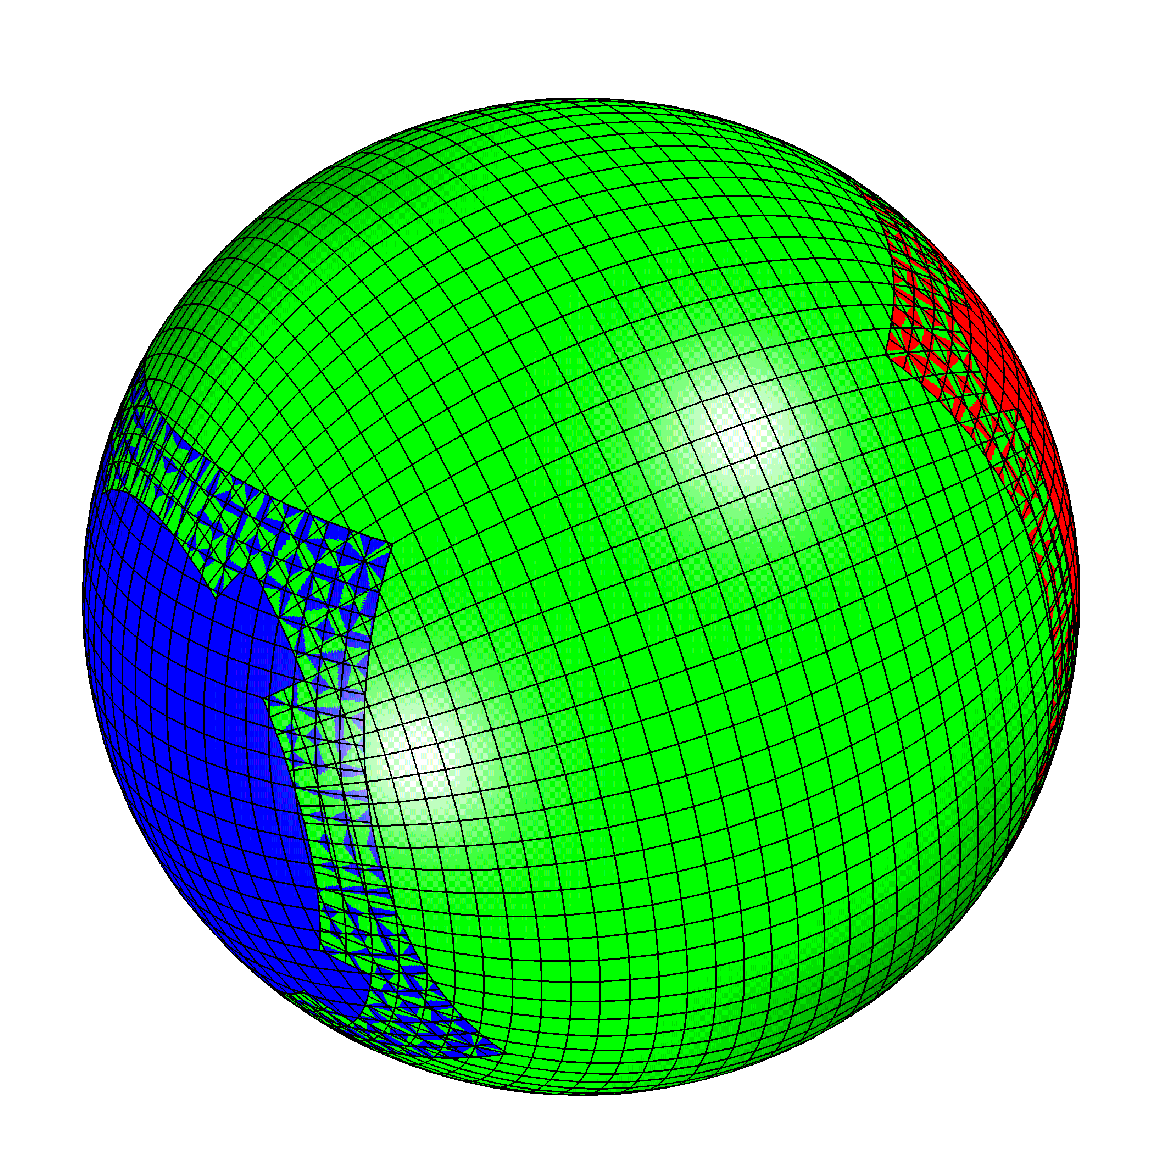
\includegraphics[width=\figWidth]{sphereEigen/solidSphere2eGrid.ps}
%* \end{center}
%*   \caption{Overlapping grid for a solid sphere consisting of two orthographic patches, a spherical polar shell and
%* an interior Cartesian grid. }
%* \label{fig:solidSphereGrid}
%* \end{figure}
%* }
%* 
%* {
%* \newcommand{\figWidth}{5.5cm}
%* \begin{figure}[hbt]
%*   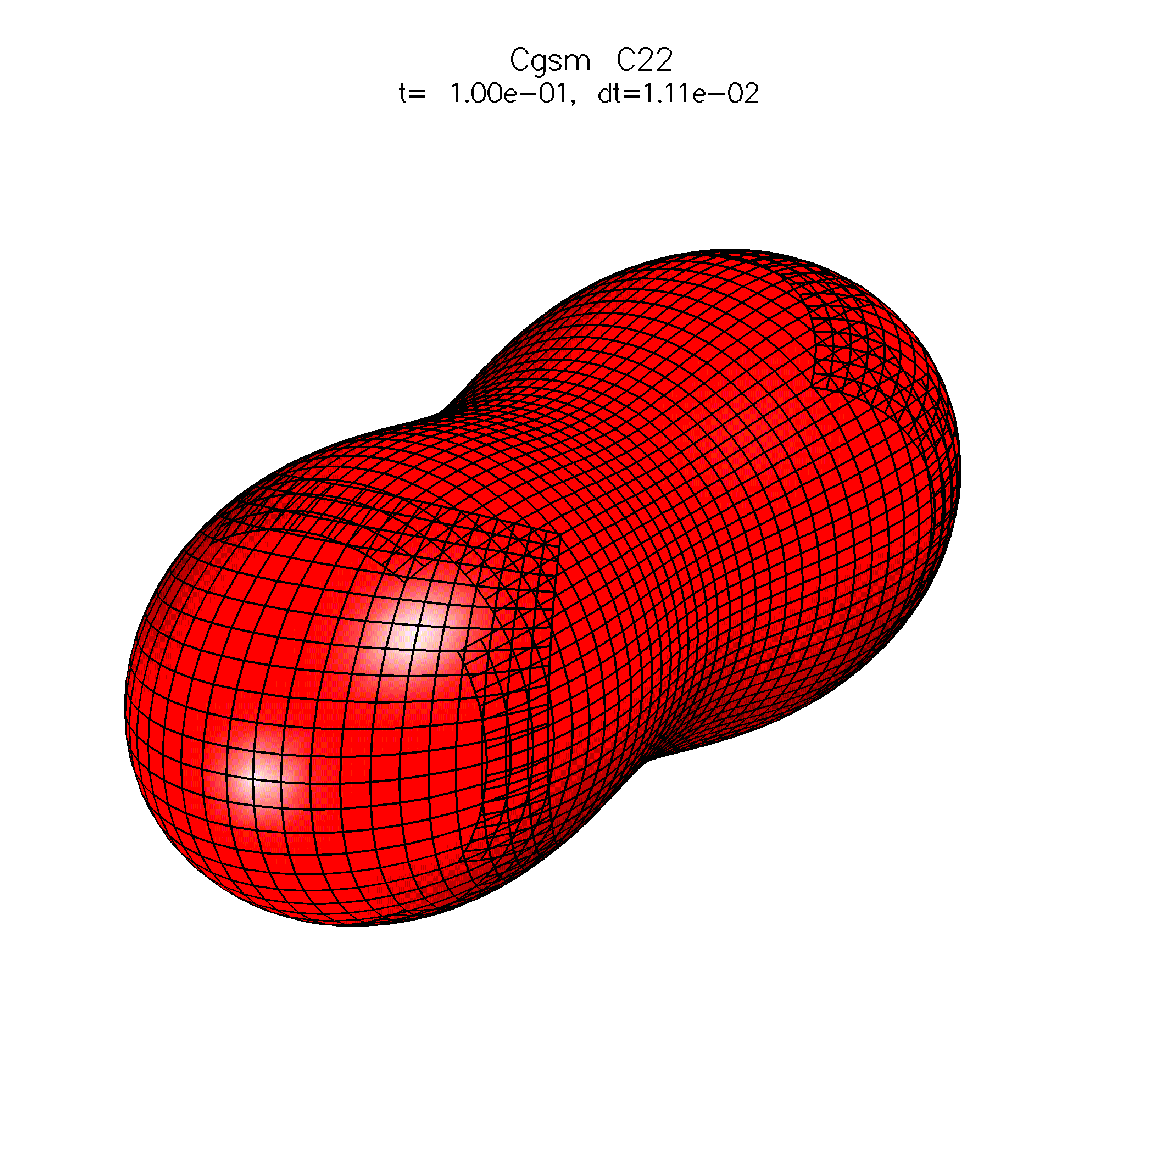
\includegraphics[width=\figWidth]{sphereEigen/sphereClassIIn2m1t1.ps}
%*   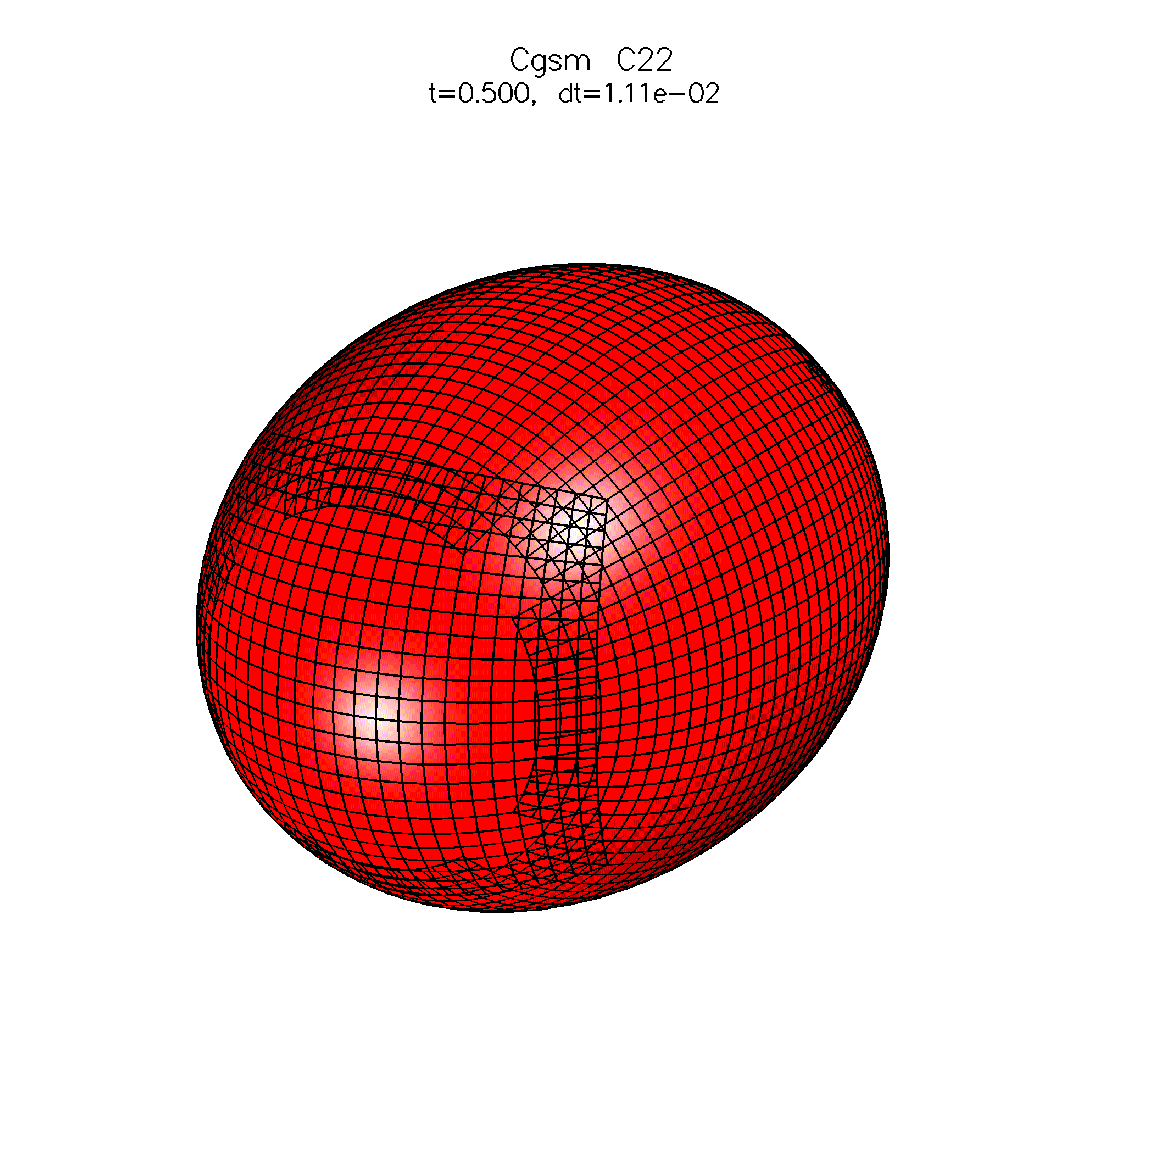
\includegraphics[width=\figWidth]{sphereEigen/sphereClassIIn2m1t5.ps}
%*   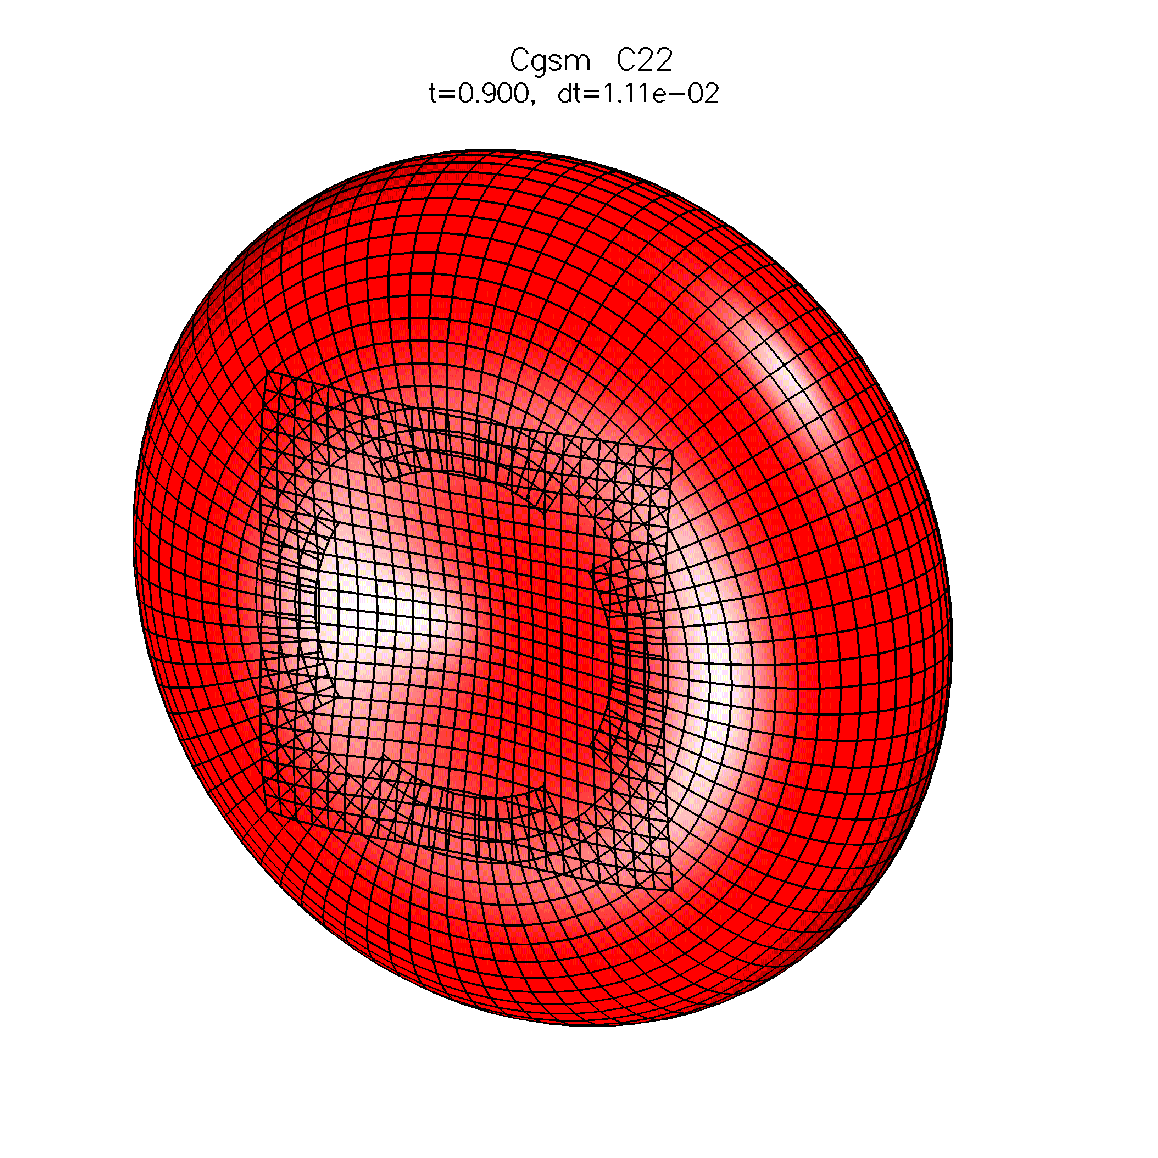
\includegraphics[width=\figWidth]{sphereEigen/sphereClassIIn2m1t9.ps}
%* % \includegraphics[width=\figWidth]{sphereEigen/sphereClassIIn2m1t13.ps}
%* % \includegraphics[width=\figWidth]{sphereEigen/sphereClassIIn2m1t17.ps}
%* % \includegraphics[width=\figWidth]{sphereEigen/sphereClassIIn2m1t21.ps}
%*   \caption{Vibration of the second class of an elastic sphere at times $t=0$, $t=0.8$ and $t=1.2$. }
%* \label{fig:sphereEigEvolution}
%* \end{figure}
%* }

%* % ----------------------------------
%* \begin{figure}[hbt]
%* \includegraphics[height=10.cm]{sphereEigen/smConvSphereClass1n1m0.eps}
%* \caption{Maximum errors in computing vibrational modes of a sphere. NOTE: Godunov results need to be finished. }
%* \label{fig:sphereEigConv}
%* \end{figure}
%* 
%* 
%* % ----------------------------------
%* \begin{figure}[hbt]
%* \includegraphics[height=10.cm]{sphereEigen/sphereClassIn1m0_u_c.ps}
%* \caption{Vibrational modes of a sphere: computed solution ...}
%* \label{fig:sphereEig}
%* \end{figure}
%* 

%* \clearpage
% ------------------------------------------------
% \subsubsection{Vibrations of the second class} 


% A second class of solutions, {\em vibrations of the second class}, is given by ...

%{\bf Note: We may need to use fixed width spherical grids to get better results.}

%{\bf Note: FOS-G: poor convergence.}
%\input sphereEigen/sphereEigen.nc.sf.class2.n2.m2.ConvTable.tex
%\input sphereEigen/sphereEigen.c.sf.class2.n2.m2.ConvTable.tex
%\input sphereEigen/sphereEigen.g.sf.class2.n2.m2.ConvTable.tex


% \clearpage
% {\bf Note: Fixed-width spherical grids give better looking convergence rates: }

% \begin{table}[hbt]\tableFont % you should set \tableFont to \footnotesize or other size
% \begin{center}
% \begin{tabular}{|l|c|c|c|} \hline 
% grid  & N &  $\vert u \vert$   & r \\ \hline 
%         sphereFixed1 &     1 & ~$1.3\times10^{ -1}$~  &            \\ \hline
%         sphereFixed2 &     2 & ~$4.0\times10^{ -2}$~  & ~$  3.2$~  \\ \hline
%         sphereFixed3 &     4 & ~$10.0\times10^{ -3}$~ & ~$  4.0$~  \\ \hline
%         sphereFixed4 &     8 & ~$2.4\times10^{ -3}$~  & ~$  4.1$~  \\ \hline
%     rate             &       &       $1.93$           &              \\ \hline
% \end{tabular}
% \caption{SM, sphereFixedEigen.c.sf.class2.n2.m1, pv=c, bcn=sf, class=2, n=2, m=1, diss=0, filter=1, filterOrder=6, filterFrequency=1, $t=0.5$, cfl=0.9, Fri Oct  2 14:18:45 2009}\label{table:sphereFixedEigen.c.sf.class2.n2.m1}
% \end{center}
% \end{table}
% \begin{table}[hbt]\tableFont % you should set \tableFont to \footnotesize or other size
% \begin{center}
% \begin{tabular}{|l|c|c|c|c|c|c|c|} \hline 
% grid  & N &  $u$  & r &  $v$  & r &  $\sigma$   & r \\ \hline 
%         sphereFixed1 &     1 & ~$5.1\times10^{ -2}$~ &           & ~$1.2\times10^{ -1}$~ &           & ~$2.6\times10^{ -1}$~ &            \\ \hline
%         sphereFixed2 &     2 & ~$1.2\times10^{ -2}$~ & ~$  4.2$~ & ~$3.0\times10^{ -2}$~ & ~$  4.0$~ & ~$5.1\times10^{ -2}$~ & ~$  5.1$~  \\ \hline
%         sphereFixed3 &     4 & ~$2.4\times10^{ -3}$~ & ~$  5.1$~ & ~$7.1\times10^{ -3}$~ & ~$  4.2$~ & ~$8.6\times10^{ -3}$~ & ~$  6.0$~  \\ \hline
%         sphereFixed4 &     8 & ~$5.2\times10^{ -4}$~ & ~$  4.6$~ & ~$1.7\times10^{ -3}$~ & ~$  4.1$~ & ~$2.0\times10^{ -3}$~ & ~$  4.3$~  \\ \hline
%     rate             &       &       $2.22$         &       &       $2.03$         &       &       $2.37$         &                        \\ \hline
% \end{tabular}
% \caption{SM, sphereFixedEigen.g.sf.class2.n2.m1, pv=g, bcn=sf, class=2, n=2, m=1, diss=0, filter=1, filterOrder=6, filterFrequency=1, $t=0.5$, cfl=0.9, Fri Oct  2 10:38:54 2009}\label{table:sphereFixedEigen.g.sf.class2.n2.m1}
% \end{center}
% \end{table}

\newcommand{\Gss}{\solidSphereGrid}
{
\renewcommand{\arraystretch}{\tablearraystretch}% increase the height of rows
\begin{table}[hbt]\tableFontSize
\begin{center}
 \begin{tabular}{|c|c|c|c|c|c|c|c|c|c|} \hline
 \multicolumn{2}{|c|}{ } & \multicolumn{2}{|c|}{SOS} & \multicolumn{6}{|c|}{FOS} \\ \hline 
 Grid ~$\Gs^{(\gm)}$ &~~$h_j$~~& $\eem_u$ & $r$ & $\eem_u$ & $r$ & $\eem_v$ & $r$  & $\eem_\sigma$  & $r$ \\ \hline 
 ~$\Gss^{(1)}$~&~1/10 ~&  ~$1.3\times10^{ -1}$~  &           & ~$5.1\times10^{ -2}$~ &           & ~$1.2\times10^{ -1}$~ &           & ~$2.6\times10^{ -1}$~ &            \\ \hline 
 ~$\Gss^{(2)}$~& 1/20  &  ~$4.0\times10^{ -2}$~  & ~$  3.2$~ & ~$1.2\times10^{ -2}$~ & ~$  4.2$~ & ~$3.0\times10^{ -2}$~ & ~$  4.0$~ & ~$5.1\times10^{ -2}$~ & ~$  5.1$~  \\ \hline 
 ~$\Gss^{(4)}$~& 1/40  &  ~$10.0\times10^{ -3}$~ & ~$  4.0$~ & ~$2.4\times10^{ -3}$~ & ~$  5.1$~ & ~$7.1\times10^{ -3}$~ & ~$  4.2$~ & ~$8.6\times10^{ -3}$~ & ~$  6.0$~  \\ \hline 
 ~$\Gss^{(8)}$~& 1/80  &  ~$2.4\times10^{ -3}$~  & ~$  4.1$~ & ~$5.2\times10^{ -4}$~ & ~$  4.6$~ & ~$1.7\times10^{ -3}$~ & ~$  4.1$~ & ~$2.0\times10^{ -3}$~ & ~$  4.3$~  \\ \hline 
 \rateLabel           &        $1.93$           &           &       $2.22$         &       &       $2.03$         &       &       $2.37$         &                        \\ \hline
 \end{tabular}
 \caption{Maximum errors and estimated convergence rates for numerical solutions of a vibrational mode of a solid sphere using the SOS and FOS schemes.}
%  \caption{Maximum errors and estimated convergence rates for computing a vibrational mode of a solid sphere. SM, sphereFixedEigen.g.sf.class2.n2.m1, pv=g, bcn=sf, class=2, n=2, m=1, diss=0, filter=1, filterOrder=6, filterFrequency=1, $t=0.5$, cfl=0.9, Fri Oct  2 10:38:54 2009}
\label{table:sphereEigen}
\end{center}
\end{table}
}

% {\bf Note: FOS-G: convergence of $\sigmav$ is degraded using linear-interpolation. Errors in $\sigmav$ are large near the interpolation boundary. Quadratic interpolation is used for the results below. }

% \input sphereEigen/sphereFixedEigen.nc.sf.class2.n2.m1.ConvTable.tex
% \input sphereEigen/sphereFixedEigen.c.sf.class2.n2.m1.ConvTable.tex
% \input sphereEigen/sphereFixedEigen.g.sf.class2.n2.m1.ConvTable.tex
